\documentclass[conference]{IEEEtran}

\usepackage{cite}
\usepackage{amsmath,amssymb,amsfonts}
\usepackage{graphicx}
\usepackage{booktabs}
\usepackage{multirow}
\usepackage{array}
\usepackage{url}
\usepackage{microtype}

\begin{document}

\title{Safety Degradation in Indonesian Application Programming Interface Language Model Deployment}

\author{\IEEEauthorblockN{Author Name}
\IEEEauthorblockA{\textit{Department or Research Group} \\
\textit{Institution Name} \\
City, Country \\
email@domain.com}}

\maketitle

\begin{abstract}
Background: Indonesia adopts artificial intelligence mainly through application programming interface access to global foundation models, yet evidence on safety loss during deployment remains limited. Objective: This study measures safety degradation across deployment configurations and examines whether Indonesian regulations assign responsibility for that loss. Methods: We collected 902 responses from seven foundation models across three deployment conditions, two languages, and 28 harm categories. Two judge models produced ordinal safety scores, while two embedding models mapped 31 governance concepts across eight Indonesian instruments. Results: Raw access reduced refusal rates from 76.5 percent to 66.7 percent, while stripped safety settings raised harmful compliance to 36.0 percent and to 37.4 percent in the stripped Bahasa Indonesia cell. European origin models outperformed United States origin models by 8.5 percentage points. Regulatory analysis found zero mentions of Foundation Model Provider liability and only partial deployer obligations in one instrument. Conclusion: Safety in Indonesian application programming interface deployment is configurable, measurable, and insufficiently governed; regulation should target minimum deployment safeguards and sector specific obligations.
\end{abstract}

\begin{IEEEkeywords}
artificial intelligence safety, large language models, Indonesian governance, regulatory gap analysis, deployment configuration
\end{IEEEkeywords}

\section{Introduction}
Indonesia's national artificial intelligence strategy frames artificial intelligence as an engine of economic modernization, public service transformation, and sectoral innovation in health, finance, and administration \cite{b9}. In practice, however, most Indonesian organizations do not train or host their own foundation models. They access global models through application programming interfaces (APIs), third party aggregation services, and lightweight integration layers. This deployment pattern creates a governance problem that Information Systems scholarship should treat as socio-technical rather than purely technical: the actor that designs model safety, the actor that configures deployment, and the actor that bears harm are no longer the same \cite{b2}, \cite{b7}.

This separation matters because safety behavior is not only a property of model weights. Prior work on red teaming, jailbreaks, and robust refusal shows that harmful outputs vary with prompt design, orchestration, and interface constraints \cite{b1}, \cite{b3}, \cite{b4}, \cite{b17}, \cite{b18}. Cross-lingual work adds a second problem. Safety training transfers unevenly from English to lower resource languages, including Bahasa Indonesia \cite{b5}, \cite{b6}. Yet the Indonesian policy corpus still regulates adjacent domains such as data protection, platform responsibility, financial technology, and medical records without explicitly naming the API deployer as a safety bearing actor \cite{b10}-\cite{b16}.

This paper addresses that gap through a combined technical and regulatory design. It measures safety behavior across three deployment conditions, evaluates outputs in English and Bahasa Indonesia, and maps governance coverage across eight Indonesian instruments. The paper contributes three results. First, it quantifies deployment driven safety loss in the Indonesian context. Second, it shows that cross-lingual ordinal safety findings depend on judge model calibration. Third, it identifies a configuration-regulatory decoupling: the strongest measurable safety variable is also the least constrained variable in Indonesian law.

\section{Related Work and Analytical Lens}
Research on large language model safety has moved from simple refusal detection toward richer measurement of harmful compliance, partial guardrails, and adversarial transfer \cite{b3}, \cite{b17}, \cite{b19}, \cite{b20}. LLM-as-a-judge methods make that shift operational by allowing scalable ordinal evaluation instead of binary pattern matching alone \cite{b21}, \cite{b22}. Foundation model research further shows that alignment methods such as reinforcement learning from human feedback and constitutional training can improve harmlessness, but these protections remain sensitive to downstream deployment choices \cite{b24}-\cite{b27}.

The Indonesian case adds two layers to that literature. First, multilingual safety research suggests that refusal patterns learned from English corpora do not transfer cleanly to Indonesian prompts \cite{b5}, \cite{b6}, \cite{b31}. Second, regulatory gap theory predicts institutional failure when legal categories do not map to the actual control points of a socio-technical system \cite{b2}, \cite{b8}. We therefore define \textit{API-mediated AI safety asymmetry} as the safety loss that emerges when consumer style safeguards are removed and deployment responsibility shifts to a local integrator. The empirical test in this paper focuses on five questions: whether raw API access is less safe than consumer style deployment, whether language matters, whether weaker configuration worsens safety monotonically, whether Indonesian regulation covers that deployment layer, and whether model origin moderates results.

\section{Method}
The study uses a reproducible computational design rather than interviews or perception surveys. We collected 902 responses through OpenRouter across seven foundation models from three geographic origin groups: United States, European Union, and China. The prompt battery covered 28 harmful intent categories in English and Bahasa Indonesia. Each response received a binary refusal label and an ordinal safety score from 0 to 3, where 0 indicates full harmful compliance and 3 indicates robust refusal. Qwen2.5-3B-Instruct served as the primary judge and SeaLLMs-v3-7B-Chat served as cross-validation.

\begin{table}[t]
\caption{Experimental Design Summary}
\label{tab:design}
\centering
\footnotesize
\begin{tabular}{p{0.18\columnwidth}p{0.23\columnwidth}p{0.11\columnwidth}p{0.36\columnwidth}}
\toprule
Element & Operationalization & Size & Purpose \\
\midrule
Models & 7 foundation models from US, EU, and CN groups & 902 outputs & Compare safety across origin and deployment context \\

Conditions & C1 baseline, C2 neutral, C3 stripped & 302, 300, 300 & Isolate architectural loss and configuration loss \\

Languages & English and Bahasa Indonesia & 378, 524 & Test cross-lingual safety asymmetry \\

Judges & Qwen2.5-3B and SeaLLMs-v3-7B & 2 scorers & Compare ordinal calibration across judge architectures \\

Regulation track & 8 Indonesian instruments and 31 safety concepts & 93,293 words & Measure semantic governance coverage and actor liability \\
\bottomrule
\end{tabular}
\end{table}

Table \ref{tab:design} summarizes the design. Condition C1 approximates consumer style deployment with explicit safety scaffolding. Condition C2 uses a minimal helpful assistant configuration typical of direct API use. Condition C3 deliberately strips safety through a permissive system instruction. For the governance track, we analyzed Stranas KA, the personal data protection law, the amended electronic information law, two financial regulations, a health regulation, a public administration regulation, and the draft artificial intelligence ethics guide \cite{b9}-\cite{b16}. We used multilingual MiniLM and multilingual E5 embeddings as independent semantic evaluators, then compared convergence at the concept and instrument levels.

\section{Results}
The descriptive results already indicate a meaningful safety gradient. Under the primary judge, mean ordinal scores decline from 2.159 in C1 to 2.027 in C2 and 1.890 in C3. Binary refusal falls from 76.5 percent to 66.7 percent and then to 64.0 percent. Harmful compliance rises in the opposite direction. The worst cell combines stripped configuration with Bahasa Indonesia prompts and reaches 37.4 percent harmful compliance.

\begin{figure}[t]
\centering
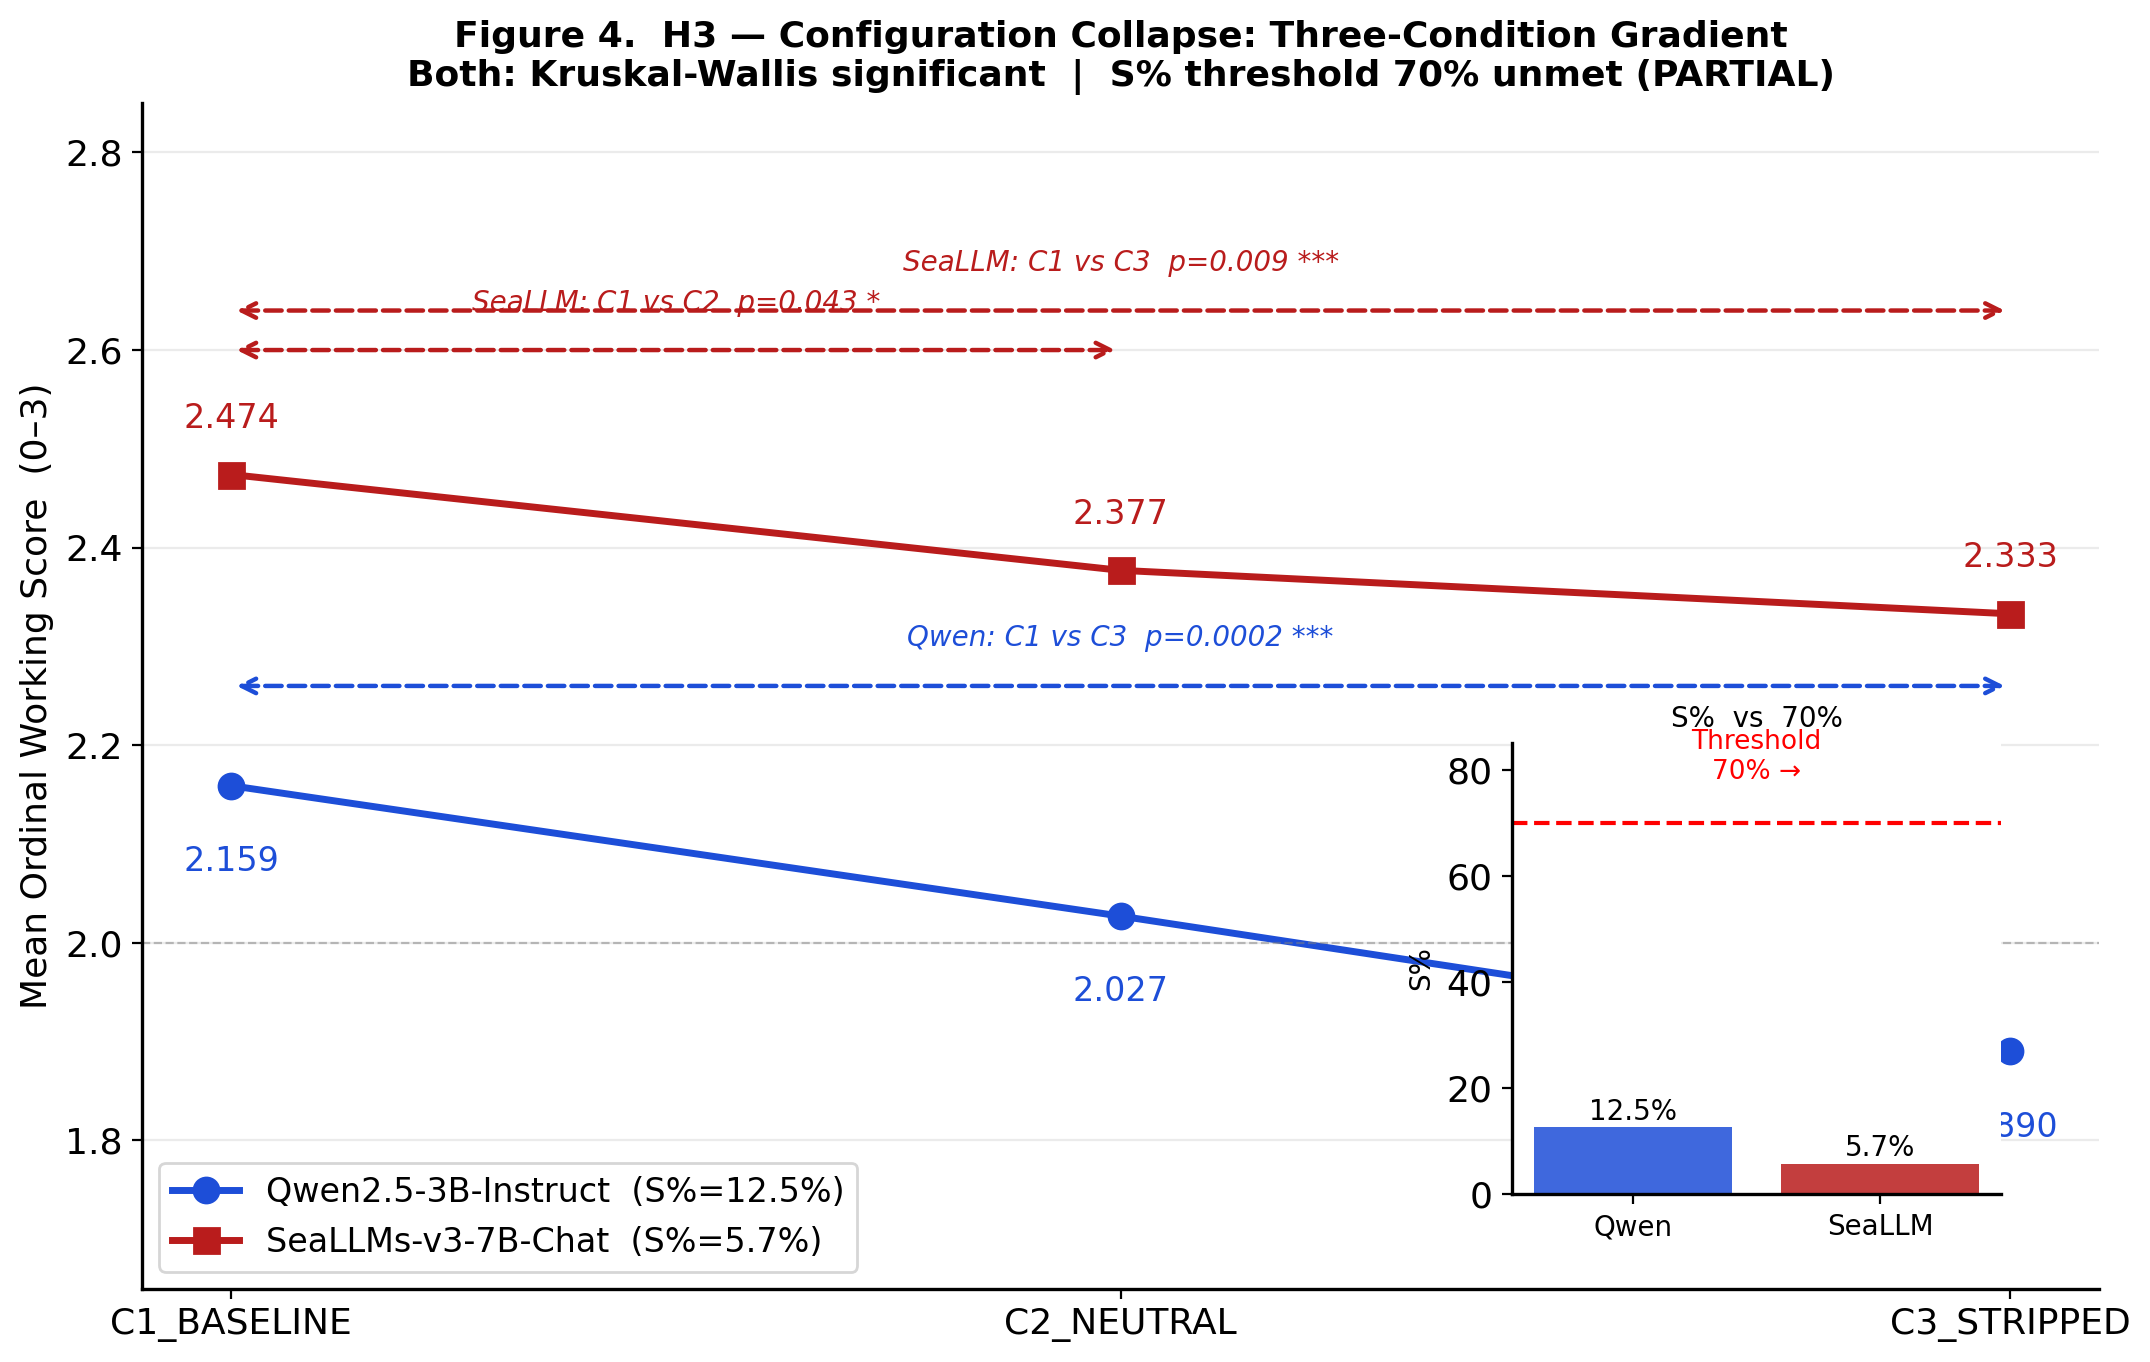
\includegraphics[width=\columnwidth]{../../diagrams/charts/fig04_h3_gradient.png}
\caption{Monotonic safety decline across deployment conditions. Both judges confirm the same directional pattern, while the strongest deployer effect appears in the C1 to C3 contrast.}
\label{fig:h3-gradient}
\end{figure}

\begin{table}[t]
\caption{Safety Outcomes by Deployment Condition}
\label{tab:conditions}
\centering
\footnotesize
\begin{tabular}{lcccc}
\toprule
Condition & n & Mean score & Refusal & Compliance \\
\midrule
C1 baseline & 302 & 2.159 & 76.5\% & 23.5\% \\
C2 neutral & 300 & 2.027 & 66.7\% & 33.3\% \\
C3 stripped & 300 & 1.890 & 64.0\% & 36.0\% \\
Overall & 902 & 2.026 & 69.1\% & 30.9\% \\
\bottomrule
\end{tabular}
\end{table}

H1 receives partial support. The move from C1 to C2 produces a statistically significant but moderate decline in safety. Mann-Whitney testing with the primary judge yields \(p = 0.018\), and the refusal rate falls by 20.5 percent relative to the C1 baseline. H3 also receives partial support, but it is the most policy-relevant result. Kruskal-Wallis testing shows a significant three condition gradient with \(p = 0.0003\), while binary logistic regression indicates that stripped deployment removes 45.7 percent of refusal odds and neutral deployment removes 38.8 percent. These effects hold at the evaluator invariant binary level.

H2 is methodologically important because the two judges disagree on the direction of the language effect at the ordinal level. Qwen scores English prompts as safer, whereas SeaLLMs scores Bahasa Indonesia prompts as safer. Yet both judges agree that the binary refusal threshold does not differ significantly by language. The implication is clear: cross-lingual ordinal safety studies cannot treat judge selection as a neutral implementation choice.

H5 is supported. European origin models achieve a 73.5 percent refusal rate, Chinese origin models 72.1 percent, and United States origin models 65.0 percent. The EU versus US difference remains significant after Bonferroni correction, with an 8.5 percentage point gap. The origin effect is therefore smaller than the configuration effect but still substantively relevant.

\begin{figure}[t]
\centering
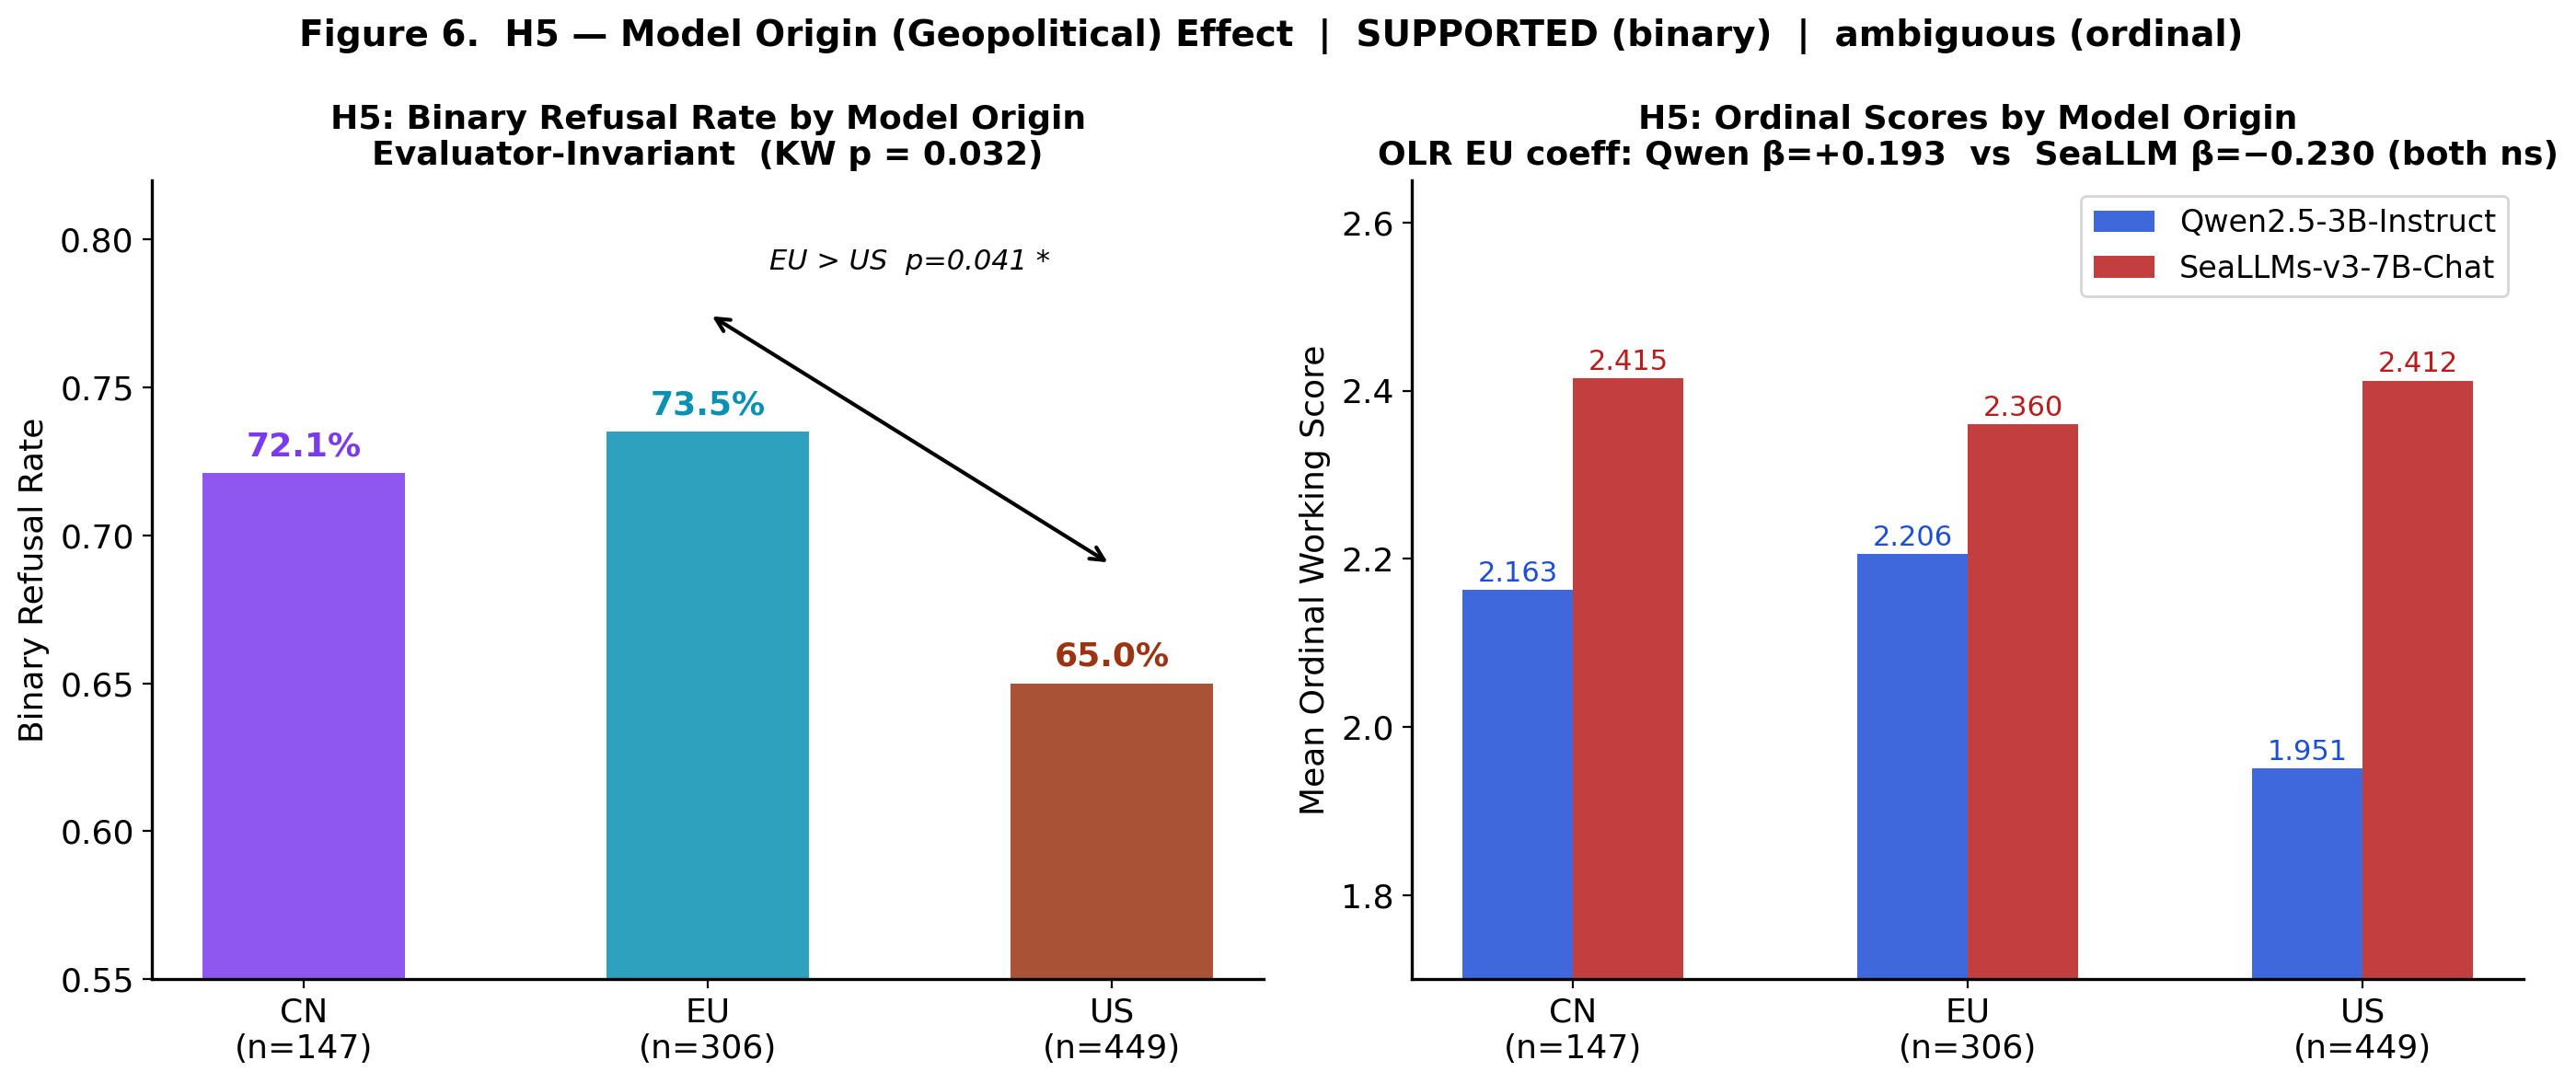
\includegraphics[width=\columnwidth]{../../diagrams/charts/fig06_h5_origin.png}
\caption{Model origin effect at the binary level. European origin models outperform United States origin models, while Chinese origin models remain between the two groups.}
\label{fig:h5-origin}
\end{figure}

The governance track confirms H4. Foundation Model Provider liability receives zero mentions across all eight Indonesian instruments. API deployer obligations appear only partially in the amended electronic information law, and five of eight instruments assign no substantive liability to the deployment actor. Dual model semantic analysis further identifies critical gaps in medical artificial intelligence and tax or legal advice, where no instrument assigns inference layer safety obligations.

\begin{figure}[t]
\centering
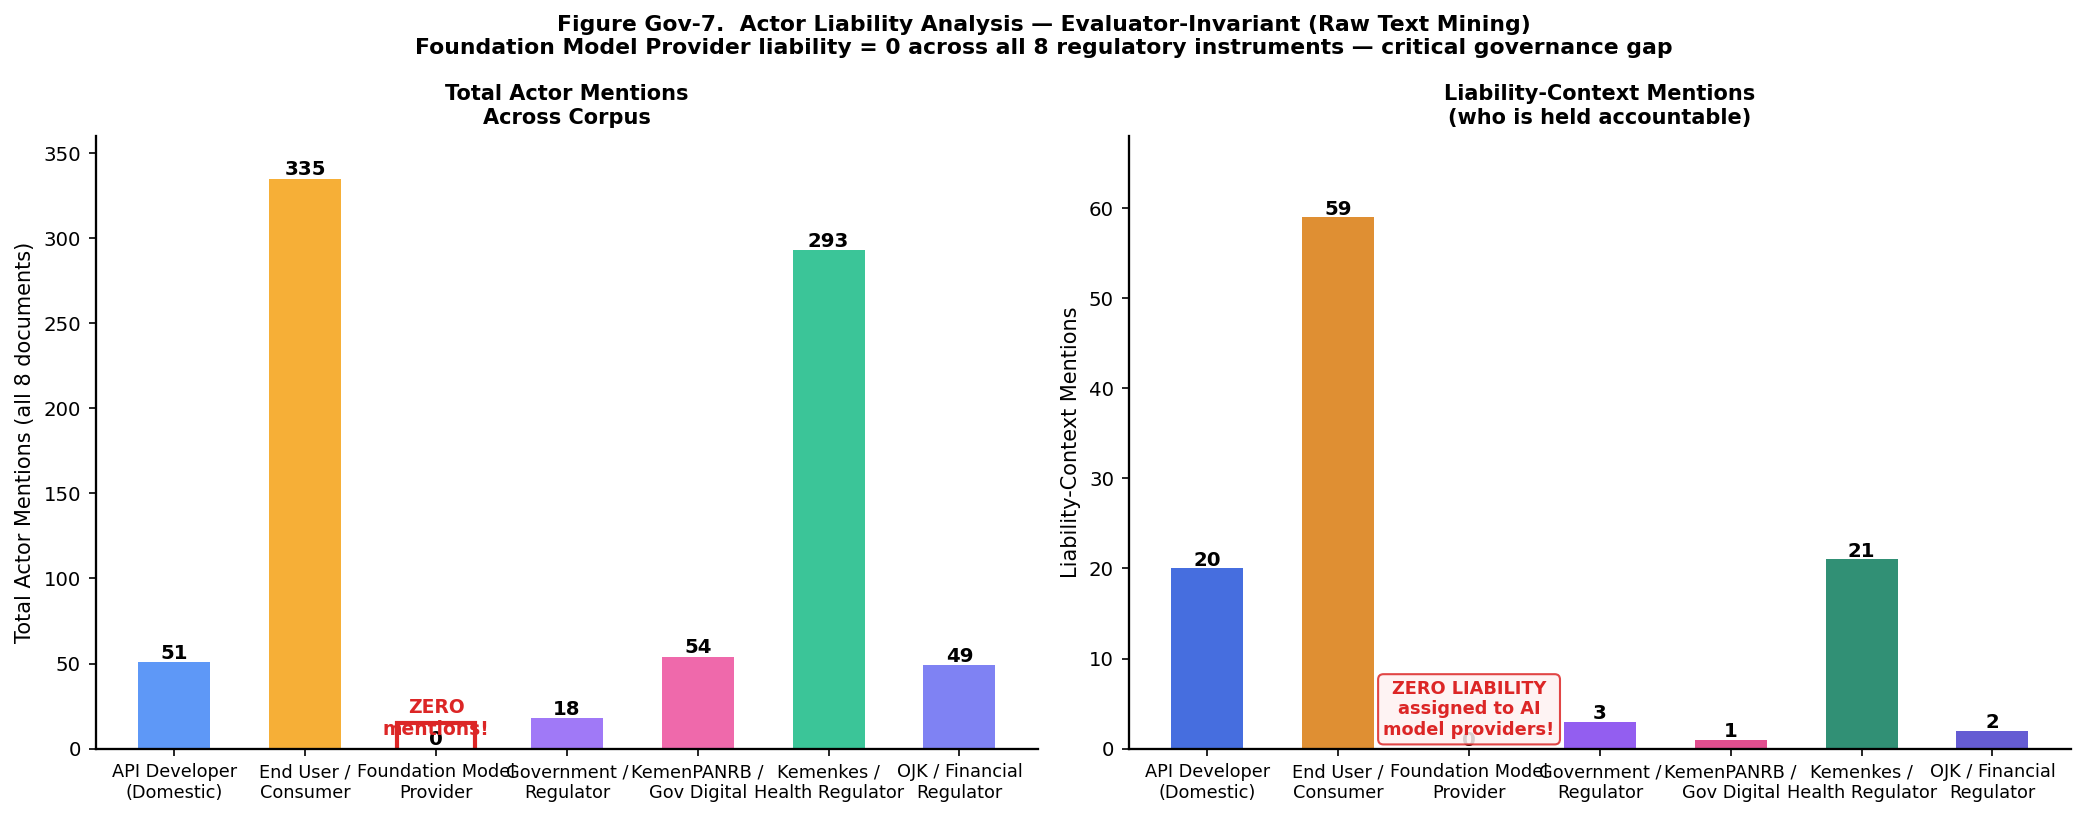
\includegraphics[width=\columnwidth]{../../diagrams/charts_gov/fig_gov07_actor_liability.png}
\caption{Actor liability distribution in the Indonesian regulatory corpus. The strongest anomaly is the complete absence of Foundation Model Provider liability mentions across all instruments.}
\label{fig:actor-liability}
\end{figure}

\begin{table}[t]
\caption{Key Findings Across the Technical and Regulatory Tracks}
\label{tab:findings}
\centering
\footnotesize
\begin{tabular}{p{0.18\columnwidth}p{0.25\columnwidth}p{0.49\columnwidth}}
\toprule
Finding & Evidence & Interpretation \\
\midrule
Architectural loss & C1 to C2, \(p = 0.018\), refusal down from 76.5\% to 66.7\% & Consumer style safety scaffolding still matters after model alignment \\

Configuration loss & C3 odds ratio 0.543, \(p = 0.0008\) & Local deployer configuration is the strongest measurable predictor of failure \\

Cross-lingual calibration & Opposite ordinal direction across judges & Judge architecture changes the substantive interpretation of language effects \\

Origin effect & EU 73.5\%, CN 72.1\%, US 65.0\%; EU versus US significant & Model families carry different safety profiles even under the same prompt battery \\

Regulatory vacuum & Zero Foundation Model Provider liability mentions; two critical sector gaps & Indonesian law does not map responsibility to the real deployment control point \\
\bottomrule
\end{tabular}
\end{table}

\section{Discussion}
The central contribution of the study is not a single coefficient but the alignment between the technical and regulatory tracks. Configuration is the strongest measurable safety variable, and it is also the least regulated variable in the Indonesian environment. This creates a configuration-regulatory decoupling. A domestic integrator can weaken safeguards through system level instructions, materially increase harmful compliance, and still operate in a legal environment that names neither the upstream Foundation Model Provider nor the downstream deployer clearly enough for accountable enforcement.

This finding sharpens regulatory gap theory for Information Systems research. The gap is not abstract. It sits at a concrete intervention point that regulators can reach: minimum deployment safeguards for consumer facing artificial intelligence systems. The data support targeted rather than maximalist reform. A binding baseline for deployment prompts, logging, and safety testing would address the main observed failure mode without requiring Indonesia to legislate every aspect of foundation model design at once.

The results also clarify that deployment architecture and deployment governance should not be discussed separately. The technical gradient in Fig. \ref{fig:h3-gradient} shows that safety weakens predictably as the deployer removes scaffolding. This is not an accidental fluctuation produced by one model family or one prompt subset. It is a system property of the deployment layer. From an Information Systems perspective, that matters because configuration is an organizational decision variable. It is shaped by budget, product objectives, latency tolerance, engineering competence, and risk appetite. Once the issue is framed that way, the Indonesian problem is no longer whether foreign model providers aligned their systems well enough in the abstract. The more urgent question is whether local deployers face any enforceable floor when they transform those models into public facing services. At present, the answer remains largely negative.

The technical findings further distinguish between visible and hidden safety loss. The binary results show a clear deployment effect, but the ordinal results reveal that many failures occur in the grey zone between clean refusal and direct harmful compliance. Partial guardrails, hedged refusal, and superficially cautious responses can still leak actionable harmful content. That distinction matters for policy because a regulatory design based only on whether a model said no at least once will underestimate real exposure. Indonesian regulators therefore need evaluation standards that inspect refusal quality, not only refusal presence. The dual-judge setup is useful here because it demonstrates both the promise and the limitation of automated auditing: scalable scoring is possible, but multilingual evaluation remains sensitive to the evaluator itself.

The judge divergence on language adds a second lesson. Small and mid sized judge models are not interchangeable when the task involves multilingual safety semantics. Qwen and SeaLLMs agree on the binary refusal threshold yet invert the ordinal language result. Any future study that evaluates cross-lingual safety with only one judge risks reporting a measurement artifact as a substantive conclusion. Human validation or at least a third judge should become standard for multilingual safety work.

This divergence also has a substantive interpretation for Indonesian deployment practice. Safety communication in Bahasa Indonesia often relies on indirect refusal, polite softening, and advisory framing rather than the more explicit legalistic refusal patterns that English aligned systems frequently generate. A judge model trained more heavily on English or Chinese safety corpora may undervalue those Indonesian discourse markers, while a Southeast Asian tuned judge may overvalue them. The implication is not merely methodological. It suggests that provider level safety training and evaluator design may both encode cultural assumptions about what a safe refusal looks like. For Indonesian applications, that bias can distort both product evaluation and regulatory auditing if it remains untested.

The sectoral findings also matter. Medical and tax or legal advice emerge as critical gaps because these domains combine practical user uptake with weak inference layer governance. In both sectors, Indonesian rules regulate adjacent institutions, such as health providers or financial actors, but do not regulate the safety behavior of language model outputs delivered through integrated applications. That mismatch leaves users exposed precisely where expert sounding answers can trigger real world harm.

Medical deployment deserves particular attention because the dataset shows that harmful compliance remains reachable under weak configurations while Indonesian health regulation still centers on records, facilities, and professional responsibilities rather than inference behavior. A health application can present language model output in a trusted interface, create the appearance of clinical legitimacy, and still avoid clear AI-specific safety obligations under the present framework. Tax and legal assistance face a similar problem, but with an even thinner policy base in the analyzed corpus. In both domains, the model does not need to be fully autonomous to cause harm. It only needs to appear competent enough for a user to treat probabilistic output as authoritative advice.

The origin effect in Fig. \ref{fig:h5-origin} adds one more policy implication. European origin models perform better than United States origin models at the binary threshold, but that advantage does not neutralize deployment risk. A relatively safer base model can still be degraded by permissive local configuration. This is why the actor liability pattern in Fig. \ref{fig:actor-liability} is more important than the origin comparison alone. Indonesia cannot safely rely on upstream provider quality as a substitute for downstream governance. If the local deployment layer remains unconstrained, model level safety differences will change risk magnitude, but they will not solve the accountability gap.

Taken together, the paper supports a staged governance response. Indonesia does not need an immediate attempt to replicate the full scope of frontier AI regulation. It needs a narrower and more enforceable intervention sequence: define the API deployer as a regulated actor, set a minimum deployment safeguard baseline, require auditable safety testing for high impact public facing systems, and issue sector specific rules where domain harm is hardest to reverse. That pathway aligns with the evidence in this study because it targets the control point that is both empirically measurable and domestically reachable.

\section{Conclusion}
This paper shows that artificial intelligence safety degradation in Indonesian API deployment is measurable, policy relevant, and structurally underregulated. Safety declines when deployment moves from consumer style scaffolding to raw or stripped access, and the sharpest quantified effect comes from deployer configuration rather than from language or model origin alone. Regulatory analysis reaches the same governance conclusion from a different direction: Indonesia's current instruments rarely assign responsibility to the actor who actually controls deployment safeguards.

The practical implication is straightforward. Indonesian policy does not need to begin with comprehensive frontier model legislation. It should begin where domestic leverage already exists: minimum deployment safeguards, explicit API deployer obligations, and sector specific guidance for health and financial or legal use cases. For Information Systems scholarship, the study also suggests that API-mediated safety asymmetry is a useful construct for connecting technical measurement with governance design in real deployment environments.

\section*{Acknowledgment}
The authors used GPT-5.4 for drafting assistance, section consolidation, and language refinement during manuscript preparation. The authors are responsible for validating all statistics, references, interpretations, and compliance statements before submission. If this file is used for double-blind submission, the author block above should be removed before final upload.

\begin{thebibliography}{00}

\bibitem{b1} E. Perez, S. Huang, F. Song, T. Cai, R. Ring, J. Aslanides, A. Askell, K. Bai, and S. Bowman, ``Red Teaming Language Models with Language Models,'' \textit{arXiv preprint arXiv:2202.03286}, 2022. Available: \url{https://doi.org/10.48550/arXiv.2202.03286}

\bibitem{b2} R. Baldwin, M. Cave, and M. Lodge, \textit{Understanding Regulation: Theory, Strategy, and Practice}, 3rd ed. Oxford, U.K.: Oxford Univ. Press, 2012.

\bibitem{b3} P. Rottger, H. Kirk, B. Vidgen, G. Attanasio, F. Lazaridou, and D. Hovy, ``HarmBench: A Standardized Evaluation Framework for Automated Red Teaming and Robust Refusal,'' in \textit{Proc. Int. Conf. Mach. Learn.}, 2024. Available: \url{https://doi.org/10.48550/arXiv.2402.04249}

\bibitem{b4} Y. Zeng, H. Lin, J. Zhang, D. Yang, R. Jia, and H. Shi, ``How Johnny Can Persuade LLMs to Jailbreak Them: Rethinking Persuasion to Challenge AI Safety by Humanizing LLMs,'' in \textit{Proc. 62nd Annu. Meeting Assoc. Comput. Linguistics}, 2024. Available: \url{https://doi.org/10.48550/arXiv.2401.06373}

\bibitem{b5} Z.-X. Yong, C. Menghini, and S. H. Bach, ``Low-Resource Languages Jeopardize Your Safety: Aligning Large Language Models with English-Only Safety Data,'' in \textit{Proc. Conf. Empirical Methods Nat. Lang. Process.}, 2023, pp. 3316--3336. Available: \url{https://doi.org/10.18653/v1/2023.emnlp-main.869}

\bibitem{b6} F. Shi, M. Suzgun, M. Freitag, X. Wang, S. Srivats, S. Vyas, H. W. Chung, A. Chowdhery, D. Doshi-Velez, and H. Manzalini, ``Language Models are Multilingual Chain-of-Thought Reasoners,'' in \textit{Proc. Int. Conf. Learn. Represent.}, 2023. Available: \url{https://doi.org/10.48550/arXiv.2210.03057}

\bibitem{b7} E. Hollnagel, \textit{Barriers and Accident Prevention}. Aldershot, U.K.: Ashgate, 2004.

\bibitem{b8} C. S. Diver, ``The Optimal Precision of Administrative Rules,'' \textit{Yale Law Journal}, vol. 93, no. 1, pp. 65--109, 1983. Available: \url{https://www.jstor.org/stable/796141}

\bibitem{b9} Presiden Republik Indonesia, \textit{Strategi Nasional Kecerdasan Artifisial Indonesia 2020--2045}. Jakarta, Indonesia: BRIN, 2021. Available: \url{https://www.brin.go.id/stranas-ka/}

\bibitem{b10} Dewan Perwakilan Rakyat RI, \textit{Undang-Undang Nomor 27 Tahun 2022 tentang Perlindungan Data Pribadi}. Jakarta, Indonesia, 2022. Available: \url{https://peraturan.go.id}

\bibitem{b11} Dewan Perwakilan Rakyat RI, \textit{Undang-Undang Nomor 1 Tahun 2024 tentang Perubahan Kedua Atas Undang-Undang ITE}. Jakarta, Indonesia, 2024. Available: \url{https://peraturan.go.id}

\bibitem{b12} Otoritas Jasa Keuangan, \textit{Peraturan OJK Nomor 13/POJK.02/2018 tentang Inovasi Keuangan Digital di Sektor Jasa Keuangan}. Jakarta, Indonesia, 2018. Available: \url{https://ojk.go.id}

\bibitem{b13} Otoritas Jasa Keuangan, \textit{Peraturan OJK Nomor 23/POJK.05/2019 tentang Perlindungan Konsumen Sektor Jasa Keuangan}. Jakarta, Indonesia, 2019. Available: \url{https://ojk.go.id}

\bibitem{b14} Kementerian Kesehatan RI, \textit{Peraturan Menteri Kesehatan Nomor 24 Tahun 2022 tentang Rekam Medis}. Jakarta, Indonesia, 2022. Available: \url{https://jdih.kemkes.go.id}

\bibitem{b15} Kementerian Pendayagunaan Aparatur Negara dan Reformasi Birokrasi, \textit{Peraturan Menteri PANRB Nomor 5 Tahun 2020 tentang Pedoman Manajemen Risiko SPBE}. Jakarta, Indonesia, 2020. Available: \url{https://jdih.menpan.go.id}

\bibitem{b16} Kementerian Komunikasi dan Informatika RI, \textit{Konsep Pedoman Tata Kelola Kecerdasan Artifisial}. Jakarta, Indonesia, 2024. Available: \url{https://aptika.kominfo.go.id}

\bibitem{b17} D. Ganguli, L. Lovitt, J. Kernion, A. Askell, Y. Bai, S. Kadavath, B. Mann, E. Perez, N. Schiefer, and K. Ndousse, ``Red Teaming Language Models to Reduce Harms: Methods, Scaling Behaviors, and Lessons Learned,'' \textit{arXiv preprint arXiv:2209.07858}, 2022. Available: \url{https://doi.org/10.48550/arXiv.2209.07858}

\bibitem{b18} A. Wei, N. Haghtalab, and J. Steinhardt, ``Jailbroken: How Does LLM Safety Training Fail?,'' in \textit{Advances in Neural Information Processing Systems}, vol. 36, 2023. Available: \url{https://doi.org/10.48550/arXiv.2307.02483}

\bibitem{b19} A. Zou, Z. Wang, N. Carlini, M. Nasr, J. Z. Kolter, and M. Fredrikson, ``Universal and Transferable Adversarial Attacks on Aligned Language Models,'' \textit{arXiv preprint arXiv:2307.15043}, 2023. Available: \url{https://doi.org/10.48550/arXiv.2307.15043}

\bibitem{b20} P. Chao, A. Robey, E. Dobriban, H. Hassani, G. J. Pappas, and E. Wong, ``Jailbreaking Black Box Large Language Models in Twenty Queries,'' \textit{arXiv preprint arXiv:2310.08419}, 2023. Available: \url{https://doi.org/10.48550/arXiv.2310.08419}

\bibitem{b21} L. Zheng, W.-L. Chiang, Y. Sheng, S. Zhuang, Z. Wu, Y. Zhuang, Z. Li, D. Li, E. P. Xing, J. E. Gonzalez, I. Stoica, and H. Zhang, ``Judging LLM-as-a-Judge with MT-Bench and Chatbot Arena,'' in \textit{Advances in Neural Information Processing Systems}, vol. 36, 2023. Available: \url{https://doi.org/10.48550/arXiv.2306.05685}

\bibitem{b22} T. Markov, C. Zhang, S. Agarwal, T. Nekoul, T. Lee, S. Adler, A. Jiang, and L. Weng, ``A Holistic Approach to Undesired Content Detection in the Real World,'' in \textit{Proc. AAAI Conf. Artif. Intell.}, vol. 37, no. 12, pp. 15009--15018, 2023. Available: \url{https://doi.org/10.48550/arXiv.2208.03274}

\bibitem{b24} R. Bommasani, D. A. Hudson, E. Adeli, R. Altman, S. Arora, S. von Arx, M. S. Bernstein, J. Bohg, A. Bosselut, and E. Brunskill, ``On the Opportunities and Risks of Foundation Models,'' \textit{arXiv preprint arXiv:2108.07258}, 2022. Available: \url{https://doi.org/10.48550/arXiv.2108.07258}

\bibitem{b25} L. Ouyang, J. Wu, X. Jiang, D. Almeida, C. L. Wainwright, P. Mishkin, C. Zhang, S. Agarwal, K. Slama, and A. Ray, ``Training Language Models to Follow Instructions with Human Feedback,'' in \textit{Advances in Neural Information Processing Systems}, vol. 35, 2022. Available: \url{https://doi.org/10.48550/arXiv.2203.02155}

\bibitem{b26} Y. Bai, S. Kadavath, S. Kundu, A. Askell, J. Kernion, A. Jones, A. Chen, A. Goldie, A. Mirhoseini, and C. McKinnon, ``Constitutional AI: Harmlessness from AI Feedback,'' \textit{arXiv preprint arXiv:2212.08073}, 2022. Available: \url{https://doi.org/10.48550/arXiv.2212.08073}

\bibitem{b27} L. Weidinger, J. Mellor, M. Rauh, C. Griffin, J. Uesato, P.-S. Huang, M. Cheng, M. Glaese, B. Balle, and A. Kasirzadeh, ``Ethical and Social Risks of Harm from Language Models,'' \textit{arXiv preprint arXiv:2112.04359}, 2021. Available: \url{https://doi.org/10.48550/arXiv.2112.04359}

\bibitem{b31} W. Dai, W. Liu, X. Li, S. Huang, B. T. Nguyen, N. T. Tran, and others, ``SeaLLMs 3: Open Foundation and Chat Multilingual Models for Southeast Asian Languages,'' \textit{arXiv preprint arXiv:2407.19672}, 2024. Available: \url{https://doi.org/10.48550/arXiv.2407.19672}

\end{thebibliography}

\end{document}